\documentclass{article}
\usepackage[utf8]{inputenc}

\usepackage[a4paper, total={6in, 8in}]{geometry}

\usepackage{natbib}
\bibliographystyle{plainnat}
\renewcommand{\bibsection}{\subsubsection*{References}}

\usepackage{graphicx}
\usepackage{url}

\bibliographystyle{abbrvnat}

%\usepackage[dvipsnames]{xcolor}

\usepackage{amsmath}
\usepackage{amsthm}
\usepackage{amssymb}

\title{The Hidden Object Data set}
\author{}
\date{} % no date

\begin{document}

\maketitle

\begin{figure}[h!]
\centering
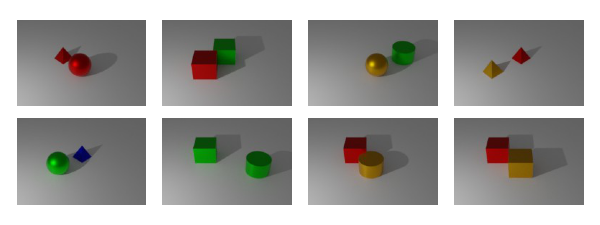
\includegraphics[width=\linewidth]{figure_hiddenObject.pdf}
\caption{Example images of the Hidden Object data set. Two objects are visible in the image, while the properties of a third `hidden' object have to predicted. (Best viewed in color.)}
\label{fig:HOsamples}
\end{figure}


The Hidden Object data set consists images containing two rendered objects, using realistic visual effects, such as shadows and reflections. The data set consists of 20,000 training images and 4,000 test images. Each object in data set is parameterized by three discrete variables: Position $\in \{ \text{middle}, \text{left}, \text{right} \}$, Color $\in \{ \text{red}, \text{green}, \text{blue}, \text{orange} \}$ and Shape $\in \{ \text{cube}, \text{cylinder}, \text{sphere}, \text{pyramid} \}$. In addition to the two observed objects, parameters for a third object are provided in tabular form. The third object can not be observed from the images, but depends via the SCM on the visible objects. The task on the data set is to infer the parameters of the third object given the $180 \times 120$ pixels image.

The DAG of the SCM is presented in Figure~\ref{fig:SCMHO}, with the following structural equations for the variables:
\[
\begin{split}
  P_1() := & \text{Categorical}([0.25, 0.5, 0.25]) \\
  C_1() := & \text{Categorical}([0.25, 0.25, 0.25, 0.25]) \\
  S_1() := & \text{Categorical}([0.25, 0.25, 0.4, 0.6]) \\
\end{split}
\]
\[
\begin{split}
  P_2(P_1) := &
  \begin{cases}
    \text{Categorical}([0.0, 0.4, 0.6]) & \text{if } P_1 = 0\\
    \text{Categorical}([0.4, 0.0, 0.6]) & \text{if } P_1 = 1\\
    \text{Categorical}([0.4, 0.6, 0.0]) & \text{if } P_1 = 2
  \end{cases} \\
  C_2(C_1, P_2) := & C_1 + P_2 + \text{Bernoulli}(0.3) \mod 4 \\
  S_2(S_3) := & S_3 \\
\end{split}
\]
\[
\begin{split}
  P_3(P_1, P_2) :=  &
  \begin{cases}
    \text{Round}((P_1 + P_2) / 2) & \text{if } \text{Rand}() < 0.98\\
    %Uniform(3) & \text{if } Rand() > 0.01\\
    0 & \text{otherwise}
  \end{cases} \\
  C_3(C_2) := & (C_2 + \text{Bernoulli}(0.1) + 3) \mod 4 \\
  S_3(S_1) := & (S_1 + \text{Categorical}([0.1, 0.8, 0.1]) + 3) \mod 4
\end{split}
\]

Data generation is performed by forward sampling from the SCM with or without a uniform intervention on one of the observed variables to yield the parameterization for the three objects. As a second step images containing the first and second objects are rendered with the blender software \citep{blender} using the previously generated parameterization. Example images are shown in Figure~\ref{fig:HOsamples}.

\begin{figure}[h!]
\centering
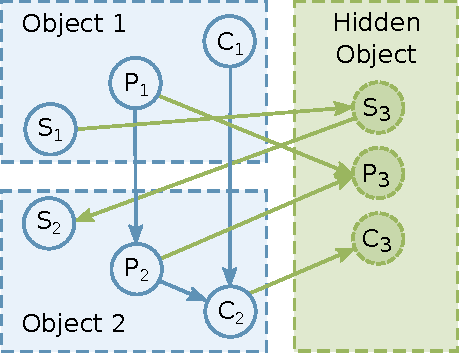
\includegraphics[width=0.35\linewidth]{figure_HiddenObjectDAG.pdf}
\caption{The DAG of the Hidden Object Data set, as induced by the structural equations. (Best viewed in color.)}
\label{fig:SCMHO}
\end{figure}



%\section*{References}
\bibliography{HiddenObjectDatasetRefs.bib}

\end{document}
